\section{Visualisierungstechniken}
Bei den Visualisierungstechniken beschäftigen wir uns vor Allem damit, wie man die Färbung Pixeln berechnen kann.

\subsection{Lineare Interpolation}

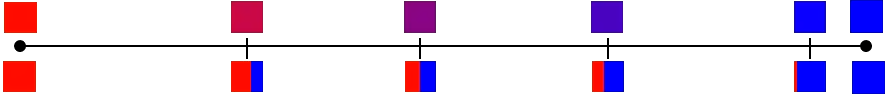
\includegraphics[width=400px]{LineareInterpolation.png}

Die lineare Interpolation beschreibt die Berechnung der Farbe eines Punktes P, der auf einer Linie liegt. Die Linie befindet sich zwischen 2 Punkten \textcolor{red}{A} und \textcolor{blue}{B} für welche die Farbe vorgegeben/bekannt ist. Jedem Punkt auf der Linie wird nun ein Anteil der Farben der Punkte A und B entsprechend seiner relativen Nähe zum jeweiligen Punkt zugeteilt.\\
Die entsprechende Rechnung ist die folgende:\\
\\
$t$ beschreibt das Verhältnis der Länge des Vektors $\overrightarrow{\mathrm{AT}}$ zur Länge des Gesamtvektors $\overrightarrow{\mathrm{AB}}$:\\
$ t = \frac{|\overrightarrow{\mathrm{AT}}|}{|\overrightarrow{\mathrm{AB}}|}$\\
$F(X)$ beschreibt die Farbe eines Punktes $X$.\\
Somit gilt nun für die Farbe des Punktes $P$:\\
\begin{math}
    F(P) = (1 - t) \cdot F(A) + t \cdot F(B)
\end{math}

\subsection{Bilineare Interpolation}

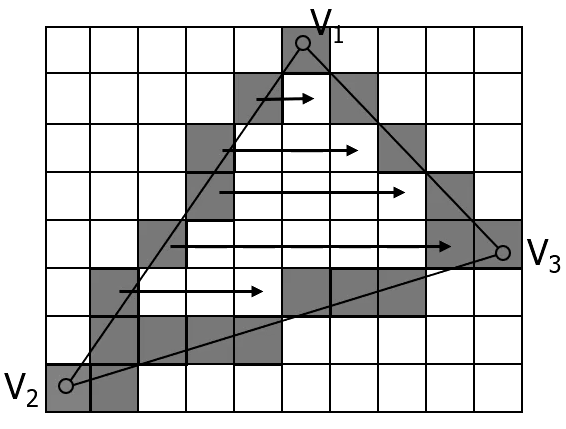
\includegraphics[width=200px]{bilineareInterpolation.png}

Die bilineare Interpolation ist ein Verfahren zur Berechnung von Farbwerten auf Flächen, die durch Eckpunkte mit vorgegebenen Farbwerten definiert werden. Dabei werden zunächst Farbwerte der Kanten durch lineare Interpolation der Eckpunkte berechnet (graue Quadrate). Danach können dann horizontal (prinzipiell könnte man das natürlich auch vertikal machen) die Farbwerte der Pixel jeder Reihe durch lineare Interpolation aus den Kanten berechnet werden (schwarze Pfeile).

\subsection{Visualisierung unter Berücksichtigung von Licht}
\subsubsection{Arten von Lichtquellen}
\textbf{Gerichtete Lichtquelle:}\\
Die Strahlen treffen parallel ein. Entsteht in der Realität annäherungsweise, wenn die Lichtquelle nahezu unendlich weit entfernt ist. Bsp.: Sonne

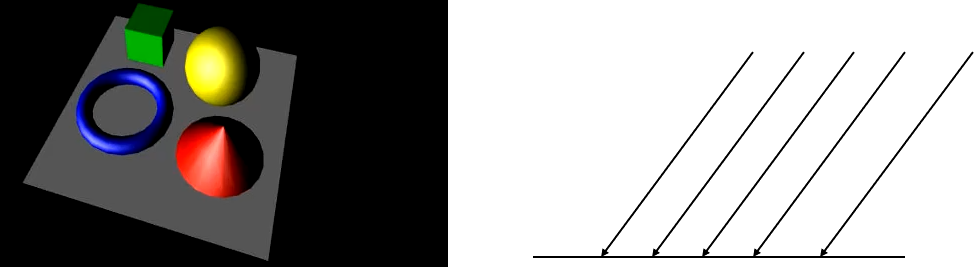
\includegraphics[width=400px]{GerichteteLichtquelle.png}

\vspace{5px}

\textbf{Punktlichtquelle:}\\
Ein Lichtquelle im lokalen Umfeld, die Strahlen in alle Richtungen abgibt. Auf diese Weise treffen Lichtstrahlen an unterschiedlichen Positionen auf einer Ebene mit unterschiedlichen Winkeln auf.

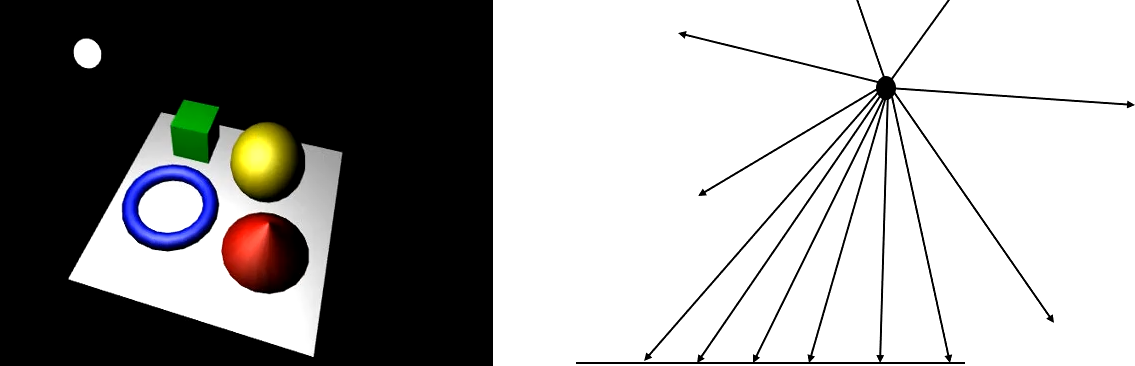
\includegraphics[width=400px]{Punktlichtquelle.png}

\vspace{5px}

\textbf{Spotlight-Lichtquelle:}\\

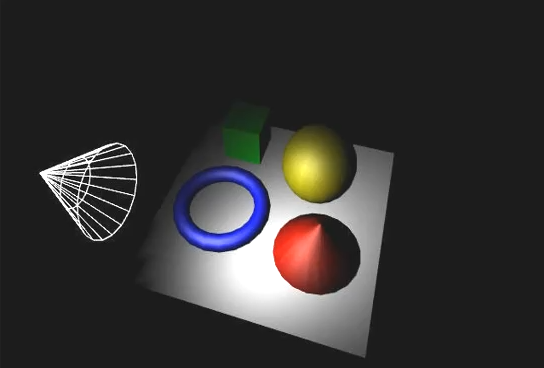
\includegraphics[width=200px]{SpotlightLichtquelle.png}

Die Strahlen kommen bezüglich des Winkels wie bei einer Punktlichtquelle an. Allerdings gibt die Lichtquelle nur in einem bestimmten Radius Licht ab. Die Lichtquelle hat also einen bestimmten Öffnungswinkel. Außerdem wird das Licht schwächer, wenn sich die Lichtquelle weiter entfernt.

\subsubsection{Phong'sches Beleuchtungsmodell}


Das Phong'sche Beleuchtungsmodell ist ein Modell, das zur Berechnung der Beleuchtung von Objekten benutzt werden kann. Dabei wird zunächst angenommen, dass die Lichtquelle Punktförmig ist. Dann werden 3 Beleuchtungsarten benutzt, deren Summe dann ein halbwegs realistisches Bild ergeben sollen:
\begin{itemize}
    \item Die \textbf{Spiegelnde Reflexion} bezeichnet die Reflexion, bei welcher der Einfallswinkel auf die Oberfläche, sowie die Position des Betrachters entscheidend sind. Hierbei entstehen bei richtigem glänzende Flächen, andernfalls bleibt die Oberfläche schwarz, da kein Licht zum Betrachter gelangt. Diese Art von Reflexion kennen wir von Spiegeln oder hochglanzpolierten Oberflächen. Das reflektierte Licht hat die hier die Farbe der der Lichtquelle.
    \item Die \textbf{Diffuse Reflexion} bezeichnet die Art von Reflexion, die man von Matten Oberflächen kennt. Dabei wird das Licht in alle Richtungen gleichermaßen reflektiert. Die diffuse Reflexion ist somit unabhängig vom Standpunkt des Betrachters. Sie ist aber abhängig vom Einfallswinkel des Lichts. Dieser bestimmt nämlich die Helligkeit der Reflexion. Das reflektierte Licht hat die hier die Farbe der Oberfläche.
    \item Die \textbf{Ambiente Reflexion} bezeichnet die Art von Reflexion, die durch eine Grundbeleuchtung der Umgebung entsteht. Die Grundbeleuchtung ist für die gesamte Szene gleich und von der Lichtquelle und dem Betrachter unabhängig. Diese Reflexion soll modellieren, dass durch wiederholte Reflexion von Licht an der Umgebung schließlich die gesamte Umgebung eine Gewisse Helligkeit hat. Dies kennt man, wenn es in einem dunklen Raum nie ganz dunkel wird, da immernoch Licht von Lichtquellen in den Raum gelangen kann, die nicht in der Szene bekannt sind. Das reflektierte Licht hat die hier die Farbe der Oberfläche.
\end{itemize}

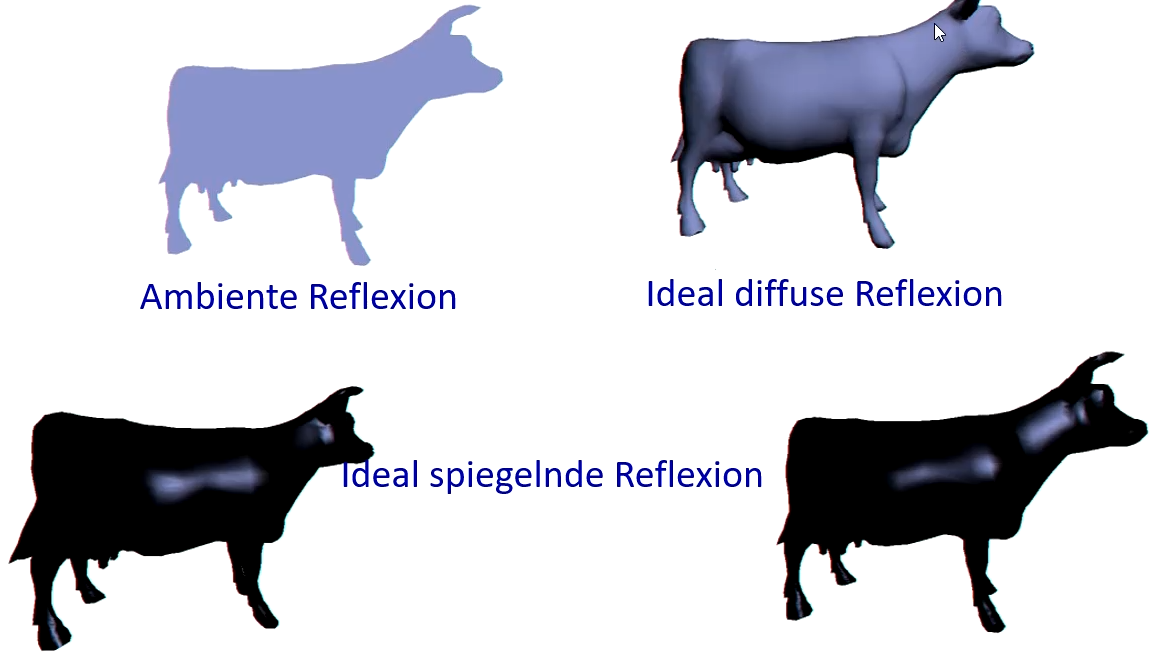
\includegraphics[width=300px]{PhongschesReflexionsmodell.png}

\subsubsection{Beleuchtungsberechnung - Methoden}
Bei der Berechnung der Beleuchtung nach dem Phong'schen sind die Winkel nötig, in denen das Licht auf die Oberfläche trifft (benötigt für spiegelnde und diffuse Reflexion). Um den Winkel berechnen zu können ist ein Normalenvektor für den Punkt/die Fläche nötig.

\vspace{10px}
\textbf{Flat Shading - Mittels Flächennormalen:}\\

\includegraphics[height=130px]{Beleuchtungsberechnung-Flächennormale-vector.png}
\hspace{15px}
\includegraphics[height=130px]{Beleuchtungsberechnung-Flächennormale.png}

Für jede Fläche wird ein Normalenvektor bestimmt. Somit wird auch für jede Fläche genau ein Eintrittswinkel und somit ein Farbwert bestimmt. Um mit dieser Berechnungsmethode ein realistisches Bild zu erschaffen benötigt man sehr viele einzelne Flächen.

\vspace{10px}
\textbf{Gouraud Shading - Mittels Eckennormalen}\\

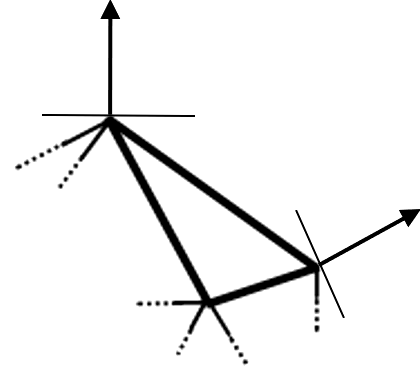
\includegraphics[height=130px]{Beleuchtungberechnung-Eckennormale-vector.png}
\hspace{150px}
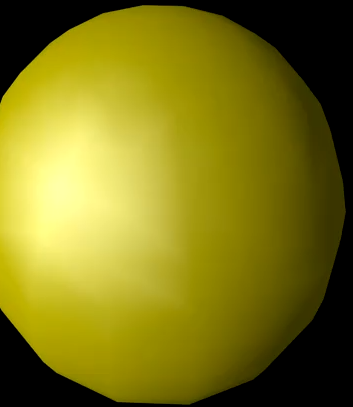
\includegraphics[height=130px]{Beleuchtungberechnung-Eckennormale.png}

Es wird ein Normalenvektor für jeden Eckpunkt der Oberfläche bestimmt. die Farbwerte der Flächen berechnen sich dann durch bilineare Interpolation der Eckpunkte. Mit dieser Methode kann recht einfach und performant ein Bild sehr realistisch Aussehen. Das Objekt selbst sieht glatt aus, Obwohl die Oberfläche aus wenigen Teilflächen besteht (Einsparung von Speicherplatz gegenüber der Benutzung von Flächennormalen mit hoher Anzahl an Flächen).\\

\begin{wrapfigure}{r}{0.35\textwidth}
    \centering
    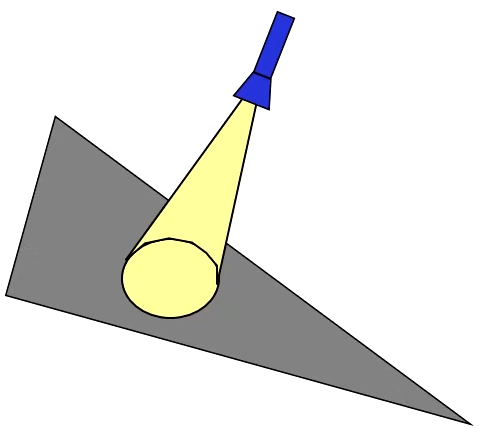
\includegraphics[height=100px]{GrenzenDesGouraudShading.png}
\end{wrapfigure}

Die \textbf{Grenze des Gouraud Shading}s ist, dass es bei sehr großen Flächen und sehr nahen Lichtquellen oder Spotlight-Lichtquellen dazu führen kann, dass die realen Farbwerte in der Mitte so verschieden zu den Farbwerten der Eckpunkte sind, dass die Fläche eine falsche Farbe erhält. Im unteren Beispiel würde so die Fläche nicht beleuchtet gerendered werden, weil ihre Eckpunkte nicht beleuchtet werden.

\vspace{10px}
\newpage
\textbf{Phong Shading - Berechnung jedes Pixels}\\
Beim Phong Shading wird für jeden Darzustellenden Pixel ein eigener Normalenvektor berechnet. Damit kann dann der Farbwert für diesen Pixel genau bestimmt werden. Mit diesem Verfahren können uns nun keine Dinge mehr entgehen, so wie es beim Gouraud Shading der Fall war. Allerdings ist die Berechnungszeit dementsprechend auch länger. Die Leistung der heutigen CPUs und GPUs hat aber dazu geführt, dass dieser Nachteil nicht mehr relevant ist.